\documentclass[a4paper]{article}

\usepackage[english]{babel}
\usepackage[T1]{fontenc}  			% make sure to install cm-super package for improved PDF quality
\usepackage[utf8]{inputenc}
%\usepackage[cm]{fullpage}			% Fullpage for now
\usepackage{graphicx}
\usepackage[dvipsnames]{xcolor}
\usepackage[font=small]{caption}
\usepackage{subcaption}
\usepackage{microtype}			 	% microtypographical fine-tunning
\usepackage{setspace} 				% Provides support for setting the spacing between lines in a document.
\usepackage{tocbibind}				% Add bibliography/index/contents to Table of Contents.
\usepackage{mathtools}				% enhances amsmath (no need to load amsmath)
\usepackage{amssymb}
\usepackage{amsfonts}
\usepackage{amsthm}
\usepackage{bm} 					% bold math symbols including greek letters
\usepackage{booktabs}				% professional tables (w/o vertical bars)
\usepackage{array}					% 
\usepackage{dcolumn} 				% align to decimal point in tables
\usepackage[shortcuts]{extdash} 	% hyphenation of dashed words
\usepackage[algoruled]{algorithm2e}
\newcommand\mycommfont[1]{\small\ttfamily #1}
\SetCommentSty{mycommfont}
\usepackage{cleveref}				% clever environment referencing
\crefname{figure}{Fig.}{Figs.}
\crefname{algorithm}{Alg.}{Algs.}
\usepackage{siunitx}				% typesetting of SI units
%\usepackage{paralist}		     	% compact lists with more options
%\usepackage[]{todonotes}			% TODO notes
%\presetkeys{todonotes}{backgroundcolor=orange!50}{}
% Not sure which to use for bibliography
%\usepackage{cite}
%\usepackage{citesort}
\usepackage[square, sort, numbers, authoryear]{natbib}
\usepackage{pgfplots}


\begin{document}

\section{Euler's Method}\label{sec:euler_method}
It's the simplest method of numerical solution for ordinary differential equations (ODEs).
Suppose we are given the following ODE with and initial condition
\begin{equation}\label{eq:ode}
	y'(t) = f(t, y(t)), \quad y(t_0) = y_0,
\end{equation}
where \( y'(t) = \frac{\mathrm{d}y}{\mathrm{d}t} \) denotes derivative.
Derivatives with respect to time, which are common in physics, are conventionally denoted by the dot symbol. 
That is, \( \dot{y}(t) \equiv y'(t) \equiv \frac{\mathrm{d}y}{\mathrm{d}t} \).
\Cref{eq:ode} is in continuous time \( t \)\footnote{Since this is mathematics we're dealing with, the variable \( t \) does not have to represent time, of course.}.
The solution of the ODE above is a function of time \( y(t) \) for which the above equation holds.
Since we are working with computers, we can't store functions of continuous variable\footnote{Because that would take up infinite memory.} and so we need to discretize the solution.
In other words, we wanna convert it to an equation in discrete time, because it's easier to implement.

The Euler method chooses some finite time step \( h \), so that \( k \)-th discrete time step can be expressed as \( t_k = t_0 + kh \).
One step of the Euler method from \( t_k \) to \( t_{k+1}  = t_k + h \) is given by
\begin{equation}
	y_{k+1} = y_k + hf(t_k, y_k),
\end{equation}
where, obviously, \( y_k = y(t_k) \).
As you can see, the recursion can be started with \( y_0 \) at \( t_0 \), because both of these are given.
We can rewrite the Euler method as 
\begin{equation}
	\frac{y_{k+1} - y_k}{h} = f(t_k, y_k)
\end{equation}

So, for example if my equation for the change in the x-coordinate in the continuous time is given by
\begin{equation}
	\dot{x}(t) = v(t)\cos(\psi(t)),
\end{equation}
than, by application of the Euler method, the discretized version with step size \( h = \mathrm{d}t \) will look like this
\begin{equation}\label{}
	x(t_{k+1}) = x(t_{k}) + v(t_k)\cos(\psi(t_k)) \mathrm{d}t.
\end{equation}
Now, to comport with the notational conventions, we are gonna use the lower index to denote the discre time steps. Since the time steps are only distinguished by the variable \( k \), using variable \( t_k \) is a bit redundant, so we will get rid of it too.
Ultimately, we get
\begin{equation}\label{eq:ode_euler}
	x_{k+1} = x_{k} + v_k\cos(\psi_k) \mathrm{d}t.
\end{equation}

With the help of the Euler method, we have converted a \emph{differential} equation into a \emph{difference} equation.
There are plenty of other, more accurate, methods for ODE integration, such as Runge-Kuta method (see Wikipedia for more), but they are more complicated.



\section{Kinematic Bicycle Model}\label{sec:kinematic_bicycle_model}
This is the kinematic bicycle model
\begin{subequations}
\begin{align}\label{eq:kinematic_bicycle_model_continuous}
\dot{x} 	&=  v \cos(\psi + \beta) \\
\dot{y} 	&=  v \sin(\psi + \beta) \\
\dot{\psi} 	&=  \frac{v}{l_r} \sin(\beta) \\
\dot{v} 	&=  a \\
\dot{\beta} &= \arctan\left(\frac{l_r}{l_r + l_f}\tan(\delta)\right)
\end{align}
\end{subequations}
Note, that the Cartesian position \( x,\ y \), the speed\footnote{a.k.a. velocity magnitude} \( v \), the inertial heading angle \( \psi \), the angle of the current velocity \( \beta \), the steering angle \( \delta \triangleq \delta_f \) and acceleration \( a \) are all functions of time.
In ODE speak, these would be called \emph{dependent variables}, whereas \( t \) is the \emph{independent variable}.
Guess why!
The distances from the center of gravity to the rear \( l_r \) axle and to the front \( l_f \) axle are constant parameters, which vary depending on the vehicle.
The \Cref{fig:kinematic_bicycle_model}, stolen from \cite{Kong2015}, depicts the geometric meaning of the variables involved.
\begin{figure}[h]
	\centering
	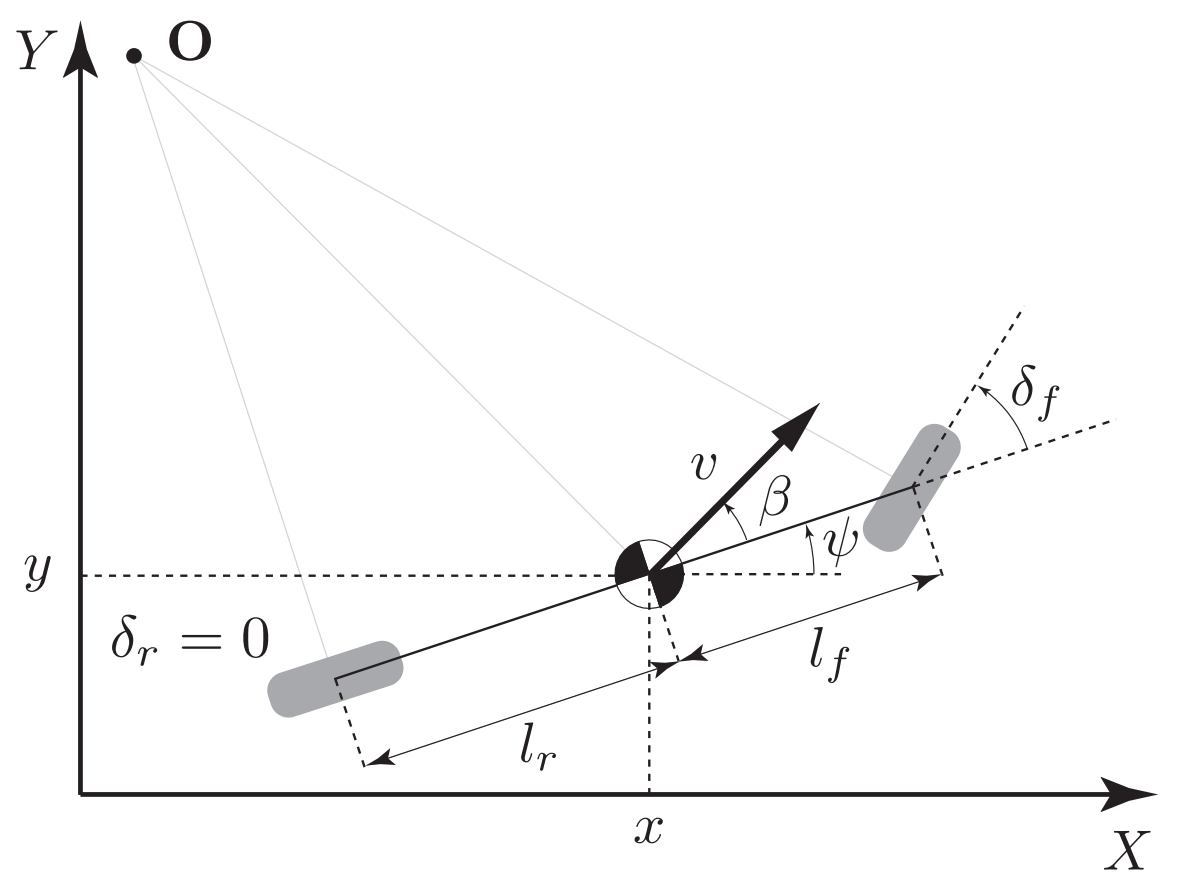
\includegraphics[scale=0.2]{./img/kinematic_bicycle_model.png}
	\caption{Kinematic bicycle model.}
	\label{fig:kinematic_bicycle_model}
\end{figure}

For some undisclosed reason, at Udacity, we are using a simplified version, given by
\begin{subequations}
\begin{align}\label{eq:kinematic_bicycle_model_continuous_udacity}
\dot{x} 	&=  v \cos(\psi) \\
\dot{y} 	&=  v \sin(\psi) \\
\dot{\psi} 	&=  \frac{v}{l_f} \delta \\
\dot{v} 	&=  a \\
\end{align}
\end{subequations}
I guess, this model assumes, among other things, that the velocity vector always points forward (in direction of the longitudinal axis of the vehicle) and the rear axle distance \( l_r = 0 \), but don't quote me on that.
Applying the Euler method from \Cref{sec:euler_method} yields the familiar equations
\begin{subequations}
\begin{align}\label{eq:kinematic_bicycle_model_discrete_udacity}
x_{k+1} 	&= x_k + v_k\cos(\psi_k) \mathrm{d}t \\
y_{k+1} 	&= y_k + v_k\sin(\psi_k) \mathrm{d}t \\
\psi_{k+1} 	&= \psi_k + \frac{v_k}{l_f}\delta_k \mathrm{d}t \\
v_{k+1} 	&= v_k + a_k\mathrm{d}t \\
\end{align}
\end{subequations}
where the \( \mathrm{d}t \) is the discretization step size.
The equations above conform to the nonlinear discrete-time state-space model in the form
\begin{equation}\label{eq:mpc_general_ssm}
	\bm{x}_{k+1} = \bm{f}(\bm{x}_k),\qquad \bm{x}_0
\end{equation}
where the state of the system is given by \( \bm{x}_k = \left[x_k,\ y_k,\ \psi_k,\ v_k \right]^\top \) and \( \bm{f}: \mathbb{R}^4\to\mathbb{R}^4 \) is the system dynamics.
The control vector \( \bm{u}_k = \left[a_k,\ \delta_k\right]^\top \) contains the system inputs; that is, the acceleration \( a_k \) and the steering angle \( \delta_k \), that influence the system state and outputs.




\section{Model Predictive Control}\label{sec:model_predictive_control}
The goal of the controller is to determine optimal values of the control variables at each time step, such that the specified optimality criteria\footnote{Such as, "don't jerk the steering wheel too fast", or "keep the speed limit while performing the maneuver", or "minimize the expended energy for actuating the control command".} are met.

Before applying the MPC algorithm, we will extend the state-space with a cross-track error \( \tilde{y}_k \) and heading error \( \tilde{\psi}_k \) variables, so that the state is now \( \bm{x}_k = \big[x_k,\ y_k,\ \psi_k,\ v_k,\ \tilde{y}_k,\ \tilde{\psi}_k \big]^\top \) and the model becomes
\begin{align}\label{eq:mpc_ssm_extended}
	x_{k+1} 			&= x_k + v_k\cos(\psi_k) \mathrm{d}t \\
	y_{k+1} 			&= y_k + v_k\sin(\psi_k) \mathrm{d}t \\
	\psi_{k+1} 			&= \psi_k + \frac{v_k}{l_f}\delta_k \mathrm{d}t \\
	v_{k+1} 			&= v_k + a_k\mathrm{d}t \\
	\tilde{y}_{k+1}		&= \tilde{y}_k + v_k\sin(\tilde{\psi}_k)\mathrm{d}t \\
	\tilde{\psi}_{k+1}	&= \tilde{\psi}_{k} + \frac{v_k}{l_f} \delta_k \mathrm{d}t
\end{align}
Let's think about error for a moment. 
Whenever we talk about error, we implicitly assume that there is some intended ground-truth value from which we departed - the error, therefore, expresses the difference between the desired (intended, reference) value and the actual value.
Let's write this formally as \( \tilde{y}_k = y_k - y^r_k \) and \( \tilde{\psi}_k = \psi_k - \psi^r_k \), where \( y^r_k \) and \( \psi^r_k \) are the reference values.
These errors arise, because the world is not perfect - actuators have their limitations, the environment is not completely predictable, the numerical noise in calculations, communication delays on the sensor network, approximative assumptions in the modeling of the vehicle motion, etc.
The reference trajectory is presumably supplied by the path planner module, which we haven't covered yet in the Term 3. 
For the purposes of the MPC project, the reference trajectory is created by fitting a polynomial to the supplied waypoints.


\textbf{Cross-Track Error} \\

\textbf{Heading Error} \\


Cross-track error
Tangential angle



Minimize cost function\footnote{Since \( J \) depends on the sequence of variables (which is a discretized function anyway), it is, strictly speaking, a \emph{functional}.} subject to constraints\footnote{Constraints are limits on \emph{relationships} between values.}
\begin{equation}\label{key}
	u_{k:k+N} = \arg\min_{u_{k:k+N}} J(u_k),
\end{equation}
subject to constraints given by the equations of dynamics [...]


and bounds\footnote{Bounds are absolute limits on the range of values.} on the actuation variables
\begin{equation}\label{eq:mpc_actuation_bounds}
	-1 \leq \alpha \leq 1 ,\qquad \SI{-25}{\degree} \leq \delta_f \leq \SI{25}{\degree}
\end{equation}



% ==========================
\bibliographystyle{plainnat}
\bibliography{refereces}

\end{document}